\documentclass[9pt]{beamer}

% \usepackage{cmap}					% поиск в PDF
% \usepackage{mathtext} 				% русские буквы в формулах
% \usepackage[T2A]{fontenc}			% кодировка
\usepackage[T1]{fontenc}		% кодировка исходного текста
\usepackage[english]{babel}	% локализация и переносы    hyperref,,caption2
\usepackage[utf8]{inputenc}	
\usepackage{amsmath,amssymb,amsfonts,amsthm}
\usepackage{bm}
% \usepackage{graphicx}
% \usepackage{tikz}
% \usepackage[framemethod=TikZ]{mdframed} % For drawing frames and boxes\
\usepackage{minted}
\newmintinline[mypython]{python}{}
\newminted{python}{fontsize=\scriptsize, 
                   linenos,
                   numbersep=8pt,
                   gobble=4,
                   frame=lines,
                   bgcolor=backcolour,
                   framesep=3mm} 

\usepackage{listings}
% Define a custom color
\definecolor{backcolour}{rgb}{0.95,0.95,0.92}
\definecolor{codegreen}{rgb}{0,0.6,0}

\usepackage[style=apa]{biblatex}
\addbibresource{../src/bibs.bib}

% Define a custom style
% \lstdefinestyle{myStyle}{
%     backgroundcolor=\color{backcolour},   
%     commentstyle=\color{codegreen},
%     basicstyle=\ttfamily\footnotesize,
%     breakatwhitespace=false,         
%     breaklines=true,                 
%     keepspaces=true,                 
%     numbers=left,       
%     numbersep=5pt,                  
%     showspaces=false,                
%     showstringspaces=false,
%     showtabs=false,                  
%     tabsize=2,
% }

\usepackage{../src/Latyshev_style}

\definecolor{MidnightBlue}{rgb}{0.2,0.2,0.7}
\usetheme{Boadilla}
\setbeamertemplate{theorems}[numbered]
\setbeamertemplate{navigation symbols}{}
\hypersetup{pdfpagemode=FullScreen}
\setbeamertemplate{footline}
{
  \leavevmode%
  \hbox{%
  \begin{beamercolorbox}[wd=1\paperwidth,ht=2.25ex,dp=1ex,right]{date in head/foot}%
    \insertframenumber{} / \inserttotalframenumber\hspace*{2ex} 
  \end{beamercolorbox}}%
  \vskip0pt%
}

\title{Finite-element implementation of plasticity \\ using a convex optimization approach}
% \subtitle{Custom assembling of plasticity problem via FEniCSx 0.3.1.0}
\author[Latyshev A.]{ {\Large Latyshev Andrey} \\ [10mm]{\small Internship supervisor: \\ Jeremy Bleyer$^1$ \newline\\ Internship co-supervisor: \\ Corrado Maurini$^2$}  }
\institute[Navier Laboratoiry]{$^1$Navier laboratory  \\$^2$Sorbonne University}
\date{ENPC, November 21 2022} 

\begin{document}

\frame{\titlepage}

\begin{frame}
  \frametitle{Objectives}
  \begin{enumerate}
    \item Write an effective program on Python for solving plasticity problems in the FEniCSx environment 
    \item Study and implement the convex optimization approach~\footfullcite{BRUNO2020724} for solving plasticity problems
  \end{enumerate}
\end{frame}

\begin{frame}
  \frametitle{Theory of plasticity}

  Assumptions:
  \begin{enumerate}
    \item Small deformations: $\uueps = \frac{1}{2}(\nabla\uu + \nabla\uu^T)$
    \item Plane strain: $u_z = 0, \, \varepsilon_{xz} = \varepsilon_{yz} = \varepsilon_{zz} = 0$
    \item Additivity deformations property: $\uueps = \uueps^e + \uueps^p$
    \item Isotropic linear elasticity: $\uusigma = \uuuuC{} : \uueps^e = \left( 3k\uuuuJ + 2\mu\uuuuK \right) : \uueps^e,$ where $\uuuuC{}$ is the fourth-order stiffness tensor, $k = (\lambda + \frac{2}{3}\mu)$ is a bulk modulus, $\lambda$ and $\mu$ are the first and the second Lamé parameters, $\uuuuK$ and $\uuuuJ$ are the forth-order tensors associated with the deviatoric operator and a unit tensor respectively
    \item Plasticity condition taking into account linear isotropic hardening: $f(\uusigma, p) = 0$, where $p = \sqrt{\frac{2}{3}\uueps^p : \uueps^p}$ is accumulated plastic strain
    \item Associative flow rule: $\dot{\uueps}^p = \dot{\lambda} \frac{\partial f(\uusigma, p)}{\partial \uusigma}$
    \item Associative hardening law: $\dot{p} = -\dot{\lambda}\frac{\partial f(\uusigma, p)}{\partial p}$
    \item Loading/unloading conditions: $\dot{\lambda} \geq 0, \quad f(\uusigma, p) \leq 0, \quad \dot{\lambda}f(\uusigma, p) = 0$
  \end{enumerate}
\end{frame}

\begin{frame}{Cylinder expansion problem}
  \begin{align}
    \Omega &: \dv \uusigma = 0, \quad \uusigma = \uuuuC{} : \uueps^e, \\
    \partial\Omega_\text{internal} &: \uusigma \cdot \un = q \cdot \un, \\
    \partial\Omega_\text{left} &: u_x = 0, \\
    \partial\Omega_\text{bottom} &: u_y = 0, \label{eqn:cylinder_bc}  \\
    \Omega &: f(\uusigma) = \sqrt{\frac{3}{2} \uus : \uus} - \sigma_0 - Hp \leq 0.
  \end{align}
  \begin{figure}[H]
    \begin{minipage}[h]{0.49\linewidth}
        \center{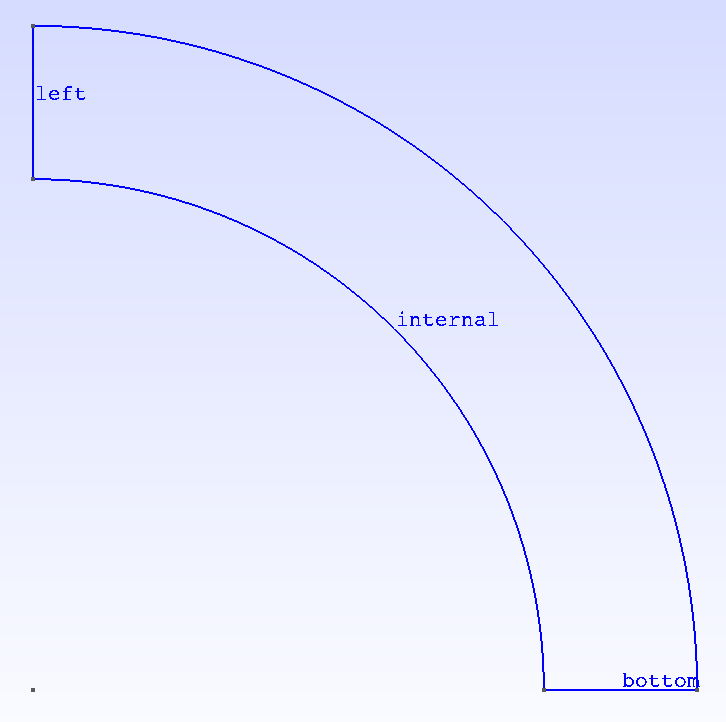
\includegraphics[width=0.6\linewidth]{../img/geometry.png} \\ Geometry}
    \end{minipage}
    \hfill
    \begin{minipage}[h]{0.49\linewidth}
        \center{\includegraphics[width=0.8\linewidth]{../img/plastic_strain.png} \\ Plastic strain on final load step}
    \end{minipage}
    \caption{Cylinder expansion problem}
    \label{fig:domain}
  \end{figure}
\end{frame}

\begin{frame}{Numerical solution of elastoplastic constitutive equations}
  Admissible displacements space:
  \begin{equation}
      V = \{\uu = (u_x, u_y) \in H^1(\Omega) \, | \, \uu = \uu_D \text{ on } \partial\Omega_D \},
  \end{equation}
  where $H^1(\Omega)$ is the first-order Sobolev space, $\uu_D$ is a displacements vector of Dirichlet boundary conditions.
  \newline 

  Variational problem:
  \begin{align}
    & \text{Find } \uu_{n+1} \in V \text{ such that,} \label{eqn:var_disc_from_1} \\ 
    & R(\uu_{n+1}) = \int\limits_\Omega\uusigman : \uueps(\uv) \, \md x - F_{n+1}^\text{ext}(\uv) = 0, \quad \forall \uv \in V \label{eqn:var_disc_from_2},
  \end{align}
  where $F_{n+1}^\text{ext}(\uv)$ is a linear form corresponding to the applied external forces, $\uusigma_{n+1} = \uusigma(\uu_{n+1})$ is a nonlinear stress tensor.
  % and $\uusigma(\uu)$ is the second-rank stress tensor, which nonlinearly depends on the displacement vector $\uu$.
  \newline 

  Linearized variational problem:
  \begin{align}
      & \text{Find } \Delta\uu \in V \text{ such that,} \label{eqn:lin_var_disc_from_1} \\ 
      & \int\limits_\Omega \left(\uuuuC{}_{n+1}^\text{tang} : \uueps(\Delta\uu)\right) : \uueps(\uv) \, \md x = -\int\limits_\Omega\uusigma_{n+1} : \uueps(\uv) \, \md x + F^\text{ext}_{n+1}(\uv) \label{eqn:lin_var_disc_from_2},
  \end{align}
  where $\uuuuC{}_{n+1}^{\text{tang}} = \frac{\partial\uusigman}{\partial\Delta\uueps}$ is a the forth-rank tangent stiffness tensor on the $n+1$ loading step.
\end{frame}

\begin{frame}{Return-mapping procedure}
  \begin{enumerate}
    \item Calculate elastic predictors: $\uusigmanelas = \uusigma_n + \uuuuC{} : \Delta\uueps$ and $p^\text{elas}_{n+1} = p_n$ \label{eqn:return_mapping_begin}
    \item If $f(\uusigma^\text{elas}_{n+1}, p^\text{elas}_{n+1}) > 0$ do the projection (can be done using a Newton method):
  \end{enumerate}
  \begin{align}
    % & \uueps_{n+1}^e = \uueps_{n}^e - \Delta\uueps - \Delta\lambda\frac{\partial f}{\partial \uusigma}(\uusigmanelas, p_n), \label{eqn:eps_e_disc} \\
    & \uusigman = \uusigmanelas - \Delta\uusigma, \\
    & p_{n+1} = p_n + \Delta p, \\%\Delta\lambda\frac{\partial f}{\partial p}(\uusigmanelas, p_n), \label{eqn:p_disc} \\
    & \Delta\uueps^p = \Delta\lambda\frac{\partial f}{\partial \uusigma} (\uusigman, p_{n+1}), \\
    & \Delta p = -\Delta\lambda\frac{\partial f}{\partial p} (\uusigman, p_{n+1}), \\
    & \Delta\lambda \geq 0, \quad f(\uusigman, p_{n+1}) \leq 0, \quad \Delta\lambda\cdot f(\uusigman, p_{n+1}) = 0. \label{eqn:return_mapping_end}
  \end{align}
  \textbf{What if the function $f = f(\uusigma, p)$ is not smooth enough?}
\end{frame}

\begin{frame}{Cylinder expansion problem. von Mises plasticity. Analytical expressions}
  % \begin{align}
  %   & \text{Find } \uu_{n+1} \text{ such that} \label{eqn:cylinder_var_1} \\
  %   & \int\limits_\Omega\uusigman : \uueps(\uv) \, \md x - q_{n+1}\int\limits_{\partial\Omega_\text{internal}}\un \cdot \uv \, \md x = 0, \quad \forall \uv \in V. \label{eqn:cylinder_var_2}
  % \end{align}

  The return-mapping procedure can be performed analytically in the von Mises plasticity case:
  \begin{align}
    & \Delta p = 
    \begin{cases}
        \frac{1}{3\mu + H}, & \text{if } f(\uusigma^\text{elas}_{n+1}, p^\text{elas}_{n+1}) \geq 0,\\
        0, & \text{otherwise},
    \end{cases} \label{eqn:dp_von_mises}\\
    & \Delta\uusigma = \beta_{n+1}\uusn, \label{eqn:dsigma_von_mises} \\
    & \dfrac{\partial\uusigman}{\partial\Delta\uueps} = \uuuuC{}_{n+1}^{\text{tang}} = \uuuuC{} - 3\mu \left( \frac{3\mu}{3\mu + H} -\beta_{n+1} \right) \uuN_{n+1} \otimes \uuN_{n+1} - 2\mu\beta_{n+1}\uuuuJ \label{eqn:C_tang_von_mises}
  \end{align}
  where $\beta_{n+1} = \frac{3\mu}{\sigmaeqnelas}\Delta p$, \quad $\uuN_{n+1} = \frac{\uus^\text{elas}_{n+1}}{\uusigmanelas}$ and $H$ is an isotropic hardening modulus.

  % Linearization of the variational problem~\eqref{eqn:cylinder_var_1}--\eqref{eqn:cylinder_var_2}:
  % \begin{align}
  %     & \text{Find } \Delta\uu \in V \text{ such that,} \label{eqn:cylinder_lin_var_from_1} \\ 
  %     & \int\limits_\Omega \left( \uuuuC{}_{n+1}^\text{tang} : \uueps(\Delta\uu) \right) : \uueps(\uv) \, \md x = -\int\limits_\Omega\uusigma_{n+1} : \uueps(\uv) \, \md x + q_{n+1}\int\limits_{\partial\Omega_\text{internal}}\un \cdot \uv \, \md x, \quad \forall \uv \in V. \label{eqn:cylinder_lin_var_from_2} 
  % \end{align}

\end{frame}


\begin{frame}{Classical approach}
  We named it "classical approach" because it's based on an implementation of von Mises plasticity via FEniCS 2019 \footfullcite{bleyer2018numericaltours}.
  \newline 

  The algorithm includes following points:
  \begin{enumerate}
    \item Divide the external loading $F_\text{ext}$ on $N$ steps 
    \item For each loading step $n+1 \in {1 \dots N}$ :
    \begin{enumerate}
        \item Solve the variational problem~\eqref{eqn:var_disc_from_1}--\eqref{eqn:var_disc_from_2} using the Newton method, where for each Newton iteration:
        \begin{enumerate}
            \item Solve the linearized problem~\eqref{eqn:lin_var_disc_from_1}--\eqref{eqn:lin_var_disc_from_2} using FEM
            \item Calculate elastic predictors $\uusigmanelas = \uusigma_n + \uuuuC{} : \Delta\uueps$ and $p^\text{elas}_{n+1} = p_n$
            \item Carry out the return-mapping procedure using analytical expressions and a function \mypython{proj_sig}, if the yield condition $f(\uusigman^\text{elas}, p^\text{elas}_{n+1}) > 0$ is true
            \item Interpolate $\uuN_{n+1}$, $\uusigman$, $\Delta p$ and $\beta_{n+1}$ in a quadrature space
            \item Update $\uusigman = \uusigmanelas - \Delta\uusigma$ and $\uuuuC{}^\text{tang}_{n+1} = \uuuuC{} - 3\mu \left( \frac{3\mu}{3\mu + H} - \beta_{n+1} \right) \uuN_{n+1} \otimes \uuN_{n+1} - 2\mu\beta_{n+1}\uuuuJ$
        \end{enumerate}
        \item Update the total displacement vector $\uu_{n+1} = \uu_n + \Delta\uu$ and cumulative plastic strain $p_{n+1} = p_n + \Delta p$
    \end{enumerate}
  \end{enumerate}
\end{frame}

\begin{frame}[fragile]
  \frametitle{Classical approach: implementation}
  \begin{pythoncode}
    deg_u = 2
    deg_stress = 2
    V = fem.VectorFunctionSpace(mesh, ("CG", deg_u))
    We = ufl.VectorElement("Quadrature", mesh.ufl_cell(), degree=deg_stress, dim=4, quad_scheme='default')
    W = fem.FunctionSpace(mesh, We)

    u = fem.Function(V, name="Total_displacement")
    du = fem.Function(V, name="Iteration_correction")
    Du = fem.Function(V, name="Current_increment")
    sig = fem.Function(W, name="Current_stress")
  \end{pythoncode}

  \begin{pythoncode}
    u_ = ufl.TrialFunction(V)
    v_ = ufl.TestFunction(V)
    a_Newton = ufl.inner(sigma_tang(eps(v_)), eps(u_))*dx
    res = -ufl.inner(eps(v_), as_3D_tensor(sig))*dx + F_ext(v_)
    my_problem = pf.LinearProblem(a_Newton, res, Du, bcs)
  \end{pythoncode}

  \begin{pythoncode}
    deps = eps(Du)
    sig_, N_, beta_, dp_ = proj_sig(deps, sig_old, p)
    fs.interpolate_quadrature(sig_, sig)
    fs.interpolate_quadrature(N_, N)
    fs.interpolate_quadrature(beta_, beta)
  \end{pythoncode}

\end{frame}

\begin{frame}{Yield criteria}
  
  Typical yield criteria
  \begin{equation}\label{eqn:yield_criterion}
    f(\uusigma, p, \sigma_C, \sigma_T, \dots) \leq 0, 
  \end{equation}
  where $\sigma_T$ and $\sigma_C$ are tensile and compressive strengths of material, respectively. 
  \newline 
  
  \textbf{von Mises criterion}:
  \begin{equation}
    \sigma_\text{eq} \leq r(\sigma_0, p),
  \end{equation}
  where $\sigma_\text{eq} = \sqrt{\frac{3}{2}\uus : \uus}$, $r(\sigma_0, p) = \sigma_0 + Hp$ represents linear isotropic hardening, where $H$ is an isotropic hardening modulus.
  \newline 
  
  \textbf{Drucker-Prager criterion}: 
  \begin{equation}
    \sigma_\text{eq} + \alpha\mtr\uusigma \leq r(\sigma_0, p),
  \end{equation}
  where $\alpha$ is a material constant.
  \newline 
  
  \textbf{Rankine criterion}:
  \begin{align*}
    & \sigma_\text{I} \leq r(\sigma_T, p), \\
    & -\sigma_\text{III} \leq r(\sigma_C, p),
  \end{align*}
  where $\sigma_\text{I} \geq \sigma_\text{II} \geq \sigma_\text{III}$ are principal stresses. 
\end{frame}

\begin{frame}{Plasticity using convex optimization}
  Let us consider the following conic optimization problem
  \begin{equation}
      \label{eqn:conic_problem}
      \begin{cases}
          \min\limits_{\uusigma, p} F(\uusigma, p), \\
          f(\uusigma, p) \leq 0,
      \end{cases}
  \end{equation}
  where the free energy $F$ of an elastoplastic material is expressed as follows
  \begin{equation}
      F(\uusigma, p) = \frac{1}{2}(\uusigmanelas - \uusigma) : \uuuuS : (\uusigmanelas - \uusigma) + \frac{1}{2}H(p_{n+1}^\text{elas} - p)^2.
  \end{equation}
  % where $H$ is an isotropic hardening modulus and $\uusigmanelas = \uusigma_n + \uuuuC{}:\Delta\uueps$ and $p^\text{elas}_{n+1} = p_n$ are elastic predictors.

  % Thus, the solution $(\uusigma^*, p^*)$ of the problem~\eqref{eqn:conic_problem} is the closest projection of $(\uusigmanelas, p_{n+1}^\text{elas})$ on the yield surface with respect to the distance induced by $\uuuuS$ and $H$, i.e. $(\uusigma_{n+1}, p_{n+1})$.
  \textbf{von Mises} and \textbf{Drucker-Prager} criteria:
  \begin{equation}
      % \label{eqn:conic_problem}
      \begin{cases}
          \min\limits_{\uusigma, p} F(\uusigma, p), \\
          \sigma_\text{eq} + \alpha\mtr\uusigma - r(\sigma_0, p) \leq 0,
      \end{cases}
  \end{equation}

  \textbf{Rankine} criterion:
  \begin{equation}
      \begin{cases}
          \min\limits_{\uusigma, p} F(\uusigma, p), \\
          \sigma_\text{I} - r(\sigma_T, p) \leq 0, \\
          -\sigma_\text{III} - r(\sigma_C, p) \leq 0.    
      \end{cases}
  \end{equation}
\end{frame}


\begin{frame}
  \frametitle{Vectorized convex optimization problem}
  \begin{itemize}
    \item $\uusigma \underset{\text{Voigt notation}}{\longrightarrow} \Sigma = (\sigma_{xx}, \sigma_{yy}, \sigma_{zz}, \sigma_{xy})^T$ 
    \item We divided Gauss nodes into patches
    \item $N_q$ Gauss nodes in total
    \item $N_\text{patch}$ Gauss nodes in one patch, where $N_\text{patch} \in [1, N_q]$
    \item $\bSigma = (\sigma_{xx}^1, \sigma_{yy}^1, \sigma_{zz}^1, \sigma_{xy}^1, \dots, \sigma_{xx}^{N_\text{patch}}, \sigma_{yy}^{N_\text{patch}}, \sigma_{zz}^{N_\text{patch}}, \sigma_{xy}^{N_\text{patch}})^T$ has a size of $4*N_\text{patch}$ components
    \item $\bP = (p^1, ..., p^{N_\text{patch}})^T$ has a size of $N_\text{patch}$ components
  \end{itemize}
  Convex optimization problem in a vectorized form:
  \begin{equation}
    % \label{eqn:conic_problem_vectorized}
    \begin{cases}
        \min\limits_{\bSigma, \bP} F(\bSigma, \bP), \\
        \mathbold{f}(\bSigma, \bP) \leq 0,
    \end{cases}
  \end{equation}
  where the vector $\mathbold{f}$ contains yield criterion $f$ values with respect to $N_\text{patch}$ Gauss nodes. 

  Free energy $F$ of an elasto-plastic material for the vectorized convex optimization problem:
  \begin{equation}
    F(\bSigma, \bP) = \frac{1}{2}(\bSigma_{n+1}^\text{elas} - \bSigma)^T \mathbb{S} (\bSigma_{n+1}^\text{elas} - \bSigma) + \frac{1}{2}H(\bP_{n+1}^\text{elas} - \bP)^T(\bP_{n+1}^\text{elas} - \bP),
  \end{equation}
  where the matrix $\mathbb{S}$ with the size $4*N_\text{patch}\times4*N_\text{patch}$ is the block-diagonal matrix with the inverted stiffness matrix $\bS$ on its diagonal.
\end{frame}

\begin{frame}{Convex plasticity}
  We call the \textit{convex plasticity} or the convex optimization approach the one where the return-mapping algorithm is implemented by solving the optimization problem.
  \newline 

  Convex optimization problem in a vectorized form:
  \begin{equation}
    \label{eqn:conic_problem_vectorized}
    \begin{cases}
        \min\limits_{\bSigma, \bP} F(\bSigma, \bP), \\
        \mathbold{f}(\bSigma, \bP) \leq 0,
    \end{cases}
  \end{equation}

  The algorithm includes following points:
  \begin{enumerate}
    \item Divide the external loading $F_\text{ext}$ on $N$ steps
    \item For each loading step $n+1 \in {1 \dots N}$:
    \begin{enumerate}
        \item Solve the variational problem~\eqref{eqn:var_disc_from_1}--\eqref{eqn:var_disc_from_2} using the \textbf{quasi-Newton method}, where for each Newton iteration:
        \begin{enumerate}
            \item Find a numerical approximation of the derivative $J = R^\prime(\uu_{n+1})$, i.e. of the linearized problem~\eqref{eqn:lin_var_disc_from_1}--\eqref{eqn:lin_var_disc_from_2}
            \item Solve the latter using FEM
            \item Calculate elastic predictors $\uusigmanelas = \uusigma_n + \uuuuC{} : \Delta\uueps$ and $p^\text{elas}_{n+1} = p_n$
            \item Carry out the return-mapping procedure by solving the conic optimization problem~\eqref{eqn:conic_problem_vectorized}, if the yield condition $f(\uusigmanelas, p^\text{elas}_{n+1}) > 0$ is true, using a \textbf{conic solver}
            % \item Update $\uuuuC{}^\text{tang}_{n+1} = \frac{\partial \uusigman}{\partial\uueps}$
            \item Update $\uusigman$ and $p_{n+1}$
        \end{enumerate}
        \item Update the total displacement vector $\uu_{n+1} = \uu_n + \Delta\uu$
    \end{enumerate}
  \end{enumerate}
\end{frame}

\begin{frame}[fragile]
  \frametitle{Implementation of solving convex problem}

  Convex optimization problem in a vectorized form:
  \begin{equation}
    \label{eqn:conic_problem_vectorized_double}
    \begin{cases}
        \min\limits_{\bSigma, \bP} F(\bSigma, \bP), \\
        \mathbold{f}(\bSigma, \bP) \leq 0,
    \end{cases}
  \end{equation}

  The proposed implementation contains following points:
  \begin{itemize}
    \item There are $\left\lfloor N_q / N_\text{patch} \right\rfloor $ patches 
    \item Solve vectorized problem~\eqref{eqn:conic_problem_vectorized_double} for each patch
    \item Solve vectorized problem for a patch with remaining $N_q \bmod N_\text{patch}$ Gauss nodes 
    \item We use the \mypython{cvxpy} library to initialize the convex problem and solve it.
    \item There are three conic solvers to be used: SCS, MOSEK, ECOS.
  \end{itemize}

\end{frame}

\begin{frame}
  \frametitle{Classical approach vs convex optimzation}

  Classical approach:
  \begin{itemize}
    \item standard Newton method (SNES or a custom one)
    \item analytical derivative $J = R^\prime(\uu_{n+1})$
    \item return-mapping procedure via analytical expressions of $\Delta\uusigma, \Delta p, \uuuuC{}^\text{tang}_{n+1}$, etc
    \item von Mises and Drucker-Prager criteria
  \end{itemize}
  
  Convex optimization:
  \begin{itemize}
    \item quasi-Newton method (SNESQN)
    \item derivative approximation $J \approx R^\prime(\uu_{n+1})$
    \item return-mapping procedure via convex optimization problem
    \item SCS, MOSEK, ECOS conic solvers 
    \item von Mises, Drucker-Prager and Rankine criteria
  \end{itemize}
\end{frame}

\begin{frame}{Custom assembling: motivation}
  \begin{align}
    & \text{Find } \uu \in V \text{ such that,} \label{eqn:var_from_1} \\ 
    & R(\uu) = \int\limits_\Omega\uusigma(\uu) : \uueps(\uv) \, \md x - F_\text{ext}(\uv) = 0, \quad \forall \uv \in V \label{eqn:var_from_2},
  \end{align}
  where an expression of $\underline{\underline{\sigma}}(\underline{u})$ is non linear for example:
  \begin{itemize}
    \item $\underline{\underline{\sigma}}(\underline{u}) = f(\varepsilon_\text{I}, \varepsilon_\text{II}, \varepsilon_\text{III})$,
    \item $\underline{\underline{\sigma}}(\underline{u}) = \underset{\alpha}{\operatorname{argmin}} g(\underline{\underline{\varepsilon}}(\underline{u}),  \alpha)$,
    \item examples of $\uusigma(\uu)$ in the previously described plasticity model.
  \end{itemize}

  Obstacles and motivations:
  \begin{enumerate}
    \item UFL is quite limited to express $\uusigma(\uu)$ or $\frac{\partial\uusigma(\uu)}{\partial\uueps} = \uuuuC{}_\text{tang}$ .
    \item We would like to avoid unnecessary memory allocation for such variables as $\beta$, $\uuN$ and others.
    \item Incorporation of external methods of a derivative calculation into assembling procedure
  \end{enumerate}
  % \begin{enumerate}
  %   \item To define nonlinear expressions of variational problems in more complex way than it's allowed by UFL
  %   \item To let an "oracle" provide values of such an expression and its derivative(s)
  %   \item To call this oracle on-the-fly during the assembly to avoid unnecessary loops, precomputations and memory allocations
% \end{enumerate}

  \textbf{Proposed solution:} change manually the assembling procedure in FEniCSx.
\end{frame}

\begin{frame}{Custom assembling: new entities}
  A new entity \mypython{CustomExpression}
  \begin{enumerate}
      \item inherits \mypython{fem.Function},
      \item contains a method \mypython{eval}, which will be called inside of the assemble loop and calculates the function local values.
  \end{enumerate}
  For instance, in the variation problem of plasticity
  \begin{equation}
    \int_\Omega \uusigma(\underline{\underline{\varepsilon}}(\underline{u})) : \underline{\underline{\varepsilon}}(\underline{v}) d\underline{x}  = 0 \quad \forall \underline{v} \in V,
  \end{equation}
  $\uusigma(\underline{\underline{\varepsilon}}(\underline{u}))$ is an example of \mypython{CustomExpression}. It contains the whole return-mapping procedure.
  \newline

  A new entity \mypython{ElementaryFunction} (or \mypython{LocalFunction}?) 
  \begin{enumerate}
      \item inherits \mypython{fem.Function}, 
      \item allocates the memory for local values only,
      \item can be updated during assembling procedure.
  \end{enumerate}
  For instance, we need the matrix $\bC^\text{tang}$ to update the bilinear part only. It would a waste of time to allocate its values in every quadrature node of every finite element. $\bC^\text{tang}$ is a good example of \mypython{ElementaryFunction}.
\end{frame}

\begin{frame}[fragile]{Custom assembling: implementation}

  \begin{itemize}
    \item A concept of jut-in-time compilation is applied.
    \item The \mypython{numba} library serves as a tool to implement this concept.
  \end{itemize}

  \begin{pythoncode}
    C_tang = ca.ElementaryFunction(QT, name='tangent') # tensor C_tang
    sig = ca.CustomExpression(W, eps(Du), [C_tang, p, dp, sig_old], get_eval) # sigma_n
  \end{pythoncode}

  \begin{pythoncode}
    def get_eval(self: ca.CustomFunction):
    tabulated_eps = self.tabulated_input_expression
    n_gauss_points = len(self.input_expression.X)
    local_shape = self.local_shape
    C_tang_shape = self.tangent.shape

    @numba.njit(fastmath=True)
    def eval(sigma_current_local, sigma_old_local, p_old_local, dp_local, coeffs_values, constants_values, coordinates, local_index, orientation):
        deps_local = np.zeros(n_gauss_points*3*3, dtype=PETSc.ScalarType)
        C_tang_local = np.zeros((n_gauss_points, *C_tang_shape), dtype=PETSc.ScalarType)
        ...
        for q in range(n_gauss_points):
            sig_n = as_3D_array(sigma_old[q])
            sig_elas = sig_n + sigma(deps_local[q])
            s = sig_elas - np.trace(sig_elas)*I/3.
            sig_eq = np.sqrt(3./2. * inner(s, s))
            f_elas = sig_eq - sig0 - H*p_old_local[q]
            f_elas_plus = ppos(f_elas)
            dp[:] = f_elas_plus/(3*mu_+H)
            
            sig_eq += TPV # for the case when sig_eq is equal to 0.0
            n_elas[:,:] = s/sig_eq*f_elas_plus/f_elas
            beta[:] = 3*mu_*dp/sig_eq
      
            new_sig = sig_elas - beta*s
            sigma_new[q][:] = np.asarray([new_sig[0, 0], new_sig[1, 1], new_sig[2, 2], new_sig[0, 1]])
            dp_local[q] = dp[0]
            
            C_tang_local[q][:] = get_C_tang(beta, n_elas)
        
        return [C_tang_local.flatten()] 
    return eval
  \end{pythoncode}
\end{frame}

\begin{frame}{Qualitative yield criterions comparison}
  \begin{figure}[H]
    \center
    \includegraphics[width=1\linewidth]{../img/yield_criterions.png}
    \caption{Displacements of the inner boundary for different yield criteria using convex plasticity approach}
  \end{figure}

  \begin{itemize}
    \item The convex optimization approach (or convex plasticity) works fine for all three yield criteria.
    \item Different values of $\alpha$ for Drucker-Prager criterion are considered.
  \end{itemize}
\end{frame}

\begin{frame}
  \frametitle{Patch size effect on the time performance of solving the conic problem}
  \begin{figure}[H]
    \center
    \includegraphics[width=1\linewidth]{../img/conic_solvers_2.png}
    % \caption{Patch size effect on the time performance of solving the conic problem: coarse mesh case}
  \end{figure}
\end{frame}

\begin{frame}{Patch size effect on the time performance of solving the conic problem}
  \begin{table}[H]
    \centering
    \begin{tabular}{|cccc|}
      \hline
      Mesh & Nodes & Elements & Gauss nodes of Q2 space \\
      \hline
      Coarse & 50	& 69 & 207 \\
      Medium & 407 & 714 & 2142 \\
      Dense & 811	& 1478 & 4434 \\
      \hline
    \end{tabular}
    \caption{Mesh data of time performance numerical tests for patch size effect}
    \label{tab:cvxpy_tests}
  \end{table}

  \begin{itemize}
    \item The larger the patch size, i.e. the larger the dimension of the vectorized conic optimization problem, the faster the program performs the calculations.
    \item Starting with a certain patch size, the program is not significantly accelerated.
    \item For large patch sizes, cvxpy expends substantial computer resources (time and RAM) to compile the optimization problem.
    \item For very dense meshes, it will not be possible to speed up the program by increasing the patch size.
    \item MOSEK works faster with problems of high dimension, but slower with small ones.
    \item ECOS is less suitable for high-dimensional problems.
    \item SCS is an optimal conic solver for problems of any dimension.
\end{itemize}
\end{frame}


% \begin{frame}
%   \frametitle{Patch size effect on the time performance of solving the conic problem: medium mesh case}
%   \begin{figure}[H]
%     \center
%     \includegraphics[width=0.7\linewidth]{../img/conic_solvers_medium.png}
%     % \caption{Patch size effect on the time performance of solving the conic problem: medium mesh case}
%   \end{figure}
% \end{frame}

% \begin{frame}
%   \frametitle{Patch size effect on the time performance of solving the conic problem: dense mesh case}

%   \begin{figure}[H]
%     \center
%     \includegraphics[width=0.7\linewidth]{../img/conic_solvers.png}
%     % \caption{Patch size effect on the time performance of solving the conic problem: dense mesh case}
%   \end{figure}
% \end{frame}

\begin{frame}
  \frametitle{Custom assembling performance}

  \begin{table}[H]
    \centering
    \begin{tabular}{|cccc|}
      \hline
      Mesh & Nodes & Elements & Gauss nodes of Q2 space \\
      \hline
      1 & 50	& 69 & 207 \\
      2 & 811 & 1478 & 4434 \\
      3 & 3706 & 7095 & 67707 \\
      4 & 11567 & 22569 & 67707 \\
      5 & 31666 & 62392 & 187176 \\
      \hline
    \end{tabular}
    \caption{Mesh data of time performance numerical tests of the custom assembling approach}
  \end{table}
\end{frame}

\begin{frame}
  \frametitle{Custom assembling performance}

  \begin{figure}[H]
    \center
    \includegraphics[width=0.7\linewidth]{../img/custom_assembling_tests.png}
    \caption{Time performance of the custom assembling approach in comparison with the classical one}
  \end{figure}

  \begin{enumerate}
    \item The compilation time of JIT overhead is negligible for high-density meshes.
    \item The custom assembling approach is slightly inferior in time to the classical one.
  \end{enumerate}

\end{frame}

\begin{frame}{Newton and quasi-Newton methods performance}
  \begin{figure}[H]
    \center
    \includegraphics[width=1\linewidth]{../img/SNES_vs_SNESQN.png}
    \caption{Performance comparison of the standard Newton method (SNES) and the quasi-Newton one (SNESQN). This is estimated for the last loading step when plastic deformations are maximal.}
    \label{fig:SNES_vs_SNESQN}
  \end{figure}
  
  \begin{itemize}
    \item Higher the mesh density, fewer iterations for the quasi-Newton method are needed.
    \item The same iterations number is needed for the Newton method convergence regardless mesh density.
    \item The program based on the quasi-Newton method spends less time than its analogue based on the standard Newton method.
    \item The \mypython{ufl.derivative} function spends more time to calculate the derivative approximation $R^\prime(\uu_{n+1})$.
  \end{itemize}
\end{frame}

\begin{frame}
  \frametitle{Conclusion}

  \begin{enumerate}
    \item An implementation of plasticity problem modeling using convex optimization problem was proposed via FEniCSx Project and the cvxpy library
    \item A framework in python was developed.
    \item Three yield criteria were taken into account: von Mises, Drucker-Prager, Rankine.
    \item A concept of custom assembling in the FEniCSx environment was extended.
    \item The custom assembling approach was compared to the classical one.
    \item A patch size effect on vectorized convex optimization problem was analyzed.
    \item Three conic solvers were used: SCS, MOSEK and ECOS.
    \item A Newton and quasi-Newton methods performance was compared.
    \item Some prospects for continuing the work were proposed.
  \end{enumerate}

\end{frame}

\begin{frame}[fragile]
  \frametitle{Prospects}

  \begin{enumerate}
    \item Results can be generalized to three-dimensional plasticity problems taking into account full-isotropic hardening law, as well as other plasticity criteria.
    \item The cvxpygen library could potentially help to combine the custom assembling approach and the convex plasticity one.
    \item It could also wrap the \mypython{derivative()} function and thus accelerate its performance. This would be useful to calculate efficiently the stress tensor derivative.
    \item This work is an open-source project, so other researchers can extend these ideas. 
  \end{enumerate}
  

\end{frame}

\begin{frame}[fragile]{Appendices. Specific variational form}
  \begin{align}
    & \text{Find } \uu_{n+1} \text{ such that} \label{eqn:cylinder_SNES_var_1} \\
    & R = \int\limits_\Omega \uusigman : \uueps(\uv) \, \md\Omega - \uF_{n+1}^\text{ext}(\uv) = \int\limits_\Omega \left( \uusigma_n + \uuuuC{} : (\Delta\uueps - \Delta\uueps^p) \right) : \uueps(\uv) \, \md\Omega - \uF_{n+1}^\text{ext}(\uv) = 0, \label{eqn:cylinder_SNES_var_2}
  \end{align}
  where $\uusigman = \uusigma(\uu_{n+1})$, $\uu_{n+1} = \uu_{n} + \Delta\uu$, $\Delta\uueps = \uueps(\Delta\uu)$ and the plastic strain increment $\Delta\uueps^p = \uueps^p(\Delta\uu)$ \textbf{actually contains a return-mapping algorithm inside}:
  \begin{equation}
      \Delta\uueps^p = 
          \begin{cases}
              \Delta p \left( \frac{3}{2}\frac{\uusnelas} {\sigmaeqnelas} \right), & \text{ if } f(\uusigmanelas, p_{n+1}) > 0,  \\
              0, & \text{ otherwise}.
          \end{cases}
  \end{equation}
  \begin{itemize}
    \item This can only be used in "analytical" cases.
    \item We calculate the derivative $J = R^\prime(\uu_{n+1})$ using \mypython{ufl.derivate()} and therefore we avoid the direct computation of $\uuuuC{}^\text{tang}_{n+1}$.
    \item It allows to use efficient SNES and SNESQN solvers.
  \end{itemize}
  \begin{pythoncode}
    residual = ufl.inner(as_3D_tensor(sig) + sigma(eps(Du) - deps_p(eps(Du), sig, p)), eps(u_))*dx - F_ext(u_)
    J = ufl.derivative(ufl.inner(sigma(eps(Du) - deps_p(eps(Du), sig, p)), eps(u_))*dx, Du, v)
    my_problem = pf.SNESProblem(residual, Du, J, bcs, petsc_options=petsc_options_SNES)
  \end{pythoncode}
\end{frame}

\begin{frame}{Appendices. Drucker-Prager plasticity model}
  \begin{equation}
    f(\uusigma, p) = \sigma_{\text{eq}} + \alpha \mtr \uusigma - R(p) \leq 0,
  \end{equation}
  \begin{equation}
    % & \sigmaeqnelas - 3\mu\Delta p + \alpha \mtr \uusigmanelas - 3\kappa 3\alpha^2 \Delta p - \sigma_0 - h p_n - h \Delta p = 0 \\
    \Delta p = \frac{ \sigmaeqnelas + \alpha \mtr \uusigmanelas - \sigma_0 - h p_n}{ \gamma },
  \end{equation}
  where $\gamma = 3\mu + 9\alpha^2\kappa + h$.

  \begin{equation}
    % & \uusigma_{n+1} = \uusigma_{n+1}^\text{elas} - 2\mu \Delta\uue^p - \kappa \mtr (\Delta\uueps^p) \uuUnit \\
    \uusigma_{n+1} = \uusigma_{n+1}^\text{elas} - \left( \beta_{n+1} \uusnelas + 3k\alpha \Delta p \uuUnit \right),
  \end{equation}
  where $\beta_{n+1} = 3\mu\frac{\Delta p}{\sigmaeqnelas}$.
  \begin{align*}
    & \uuuuC{}^\text{tang}_{n+1} = \frac{\partial\uusigman}{\partial \Delta\uueps} = \uuuuC{} - \frac{\partial (2\mu\Delta\uue^p + k\mtr\Delta\uueps^p\uuUnit)}{\partial\Delta\uueps} = \\
    & = \uuuuC{} - \left( 3\mu\left(\frac{3\mu}{\gamma} - \beta_{n+1}\right)\uuN_{n+1} \otimes \uuN_{n+1} + \frac{9\alpha\mu k}{\gamma} (\uuUnit \otimes \uuN_{n+1} + \uuN_{n+1} \otimes \uuUnit) + \frac{9\alpha^2k^2}{\gamma} \uuUnit \otimes \uuUnit + 2\mu\beta_{n+1} \uuuuK \right),
\end{align*}
where $\uuN_{n+1} = \frac{\uus^\text{elas}_{n+1}}{\sigmaeqnelas} = \frac{\uus_{n+1}}{\sigmaeqn}$.
\end{frame}



% \begin{frame}[fragile]{Problem formulation}
%   \begin{align}
%     & f(\uusigma) = \sqrt{\frac{3}{2} \uus : \uus} - \sigma_0 - H p \leq 0 \\
%     & \int_\Omega \left( \uuuuC^\text{tang} : \uueps(\ul{u})  \right) : \uueps(\ul{v}) dx + \int_\Omega \uusigma : \uueps(\ul{v}) dx + q\int_{\partial\Omega_{\text{inside}}}  \ul{n} \cdot \ul{v} dx = 0 \\
%     & \uuuuC^\text{tang} = \uuuuC - 3\mu \left( \frac{3\mu}{3\mu + H} -\beta \right) \uun \otimes \uun - 2\mu\beta \ul{\ul{\ul{\ul{DEV}}}} \\
%     & \Delta p = \frac{<f>_+}{3\mu + H}, \quad \beta = \frac{3\mu}{\sigma_\text{eq}}\Delta p, \quad \uun = \frac{\uus}{\sigma_\text{eq}} \\
%     & \partial\Omega_\text{inside} : \uusigma \, \ul{n} = q\ul{n} \\
%     & \partial\Omega_\text{left}, \partial\Omega_\text{right} : symmetry
%   \end{align}

%   \begin{pythoncode}
%     a_Newton = ufl.inner(eps(v), inner_product(sig.tangent, eps(u_)))*dx
%     res = -ufl.inner(eps(u_), as_3D_tensor(sig))*dx 
%     res_Neumann = F_ext(u_)
%   \end{pythoncode}
% \end{frame}

% \begin{frame}{FEniCSx entities and our needs}
%   Fenics has following essential entities 
%   \begin{itemize}
%     \item \mintinline{python}{fem.Constants} (form constants). Size: number of constant scalars. FEniCS uses the same ensemble of values for every element, for every node in element
%     \item \mintinline{python}{fem.Function} (form coefficients). Size: global number of DoFs * coefficient dimension $\approx$ number of cells * number of element nodes * coefficient dimension
%     \item \mintinline{python}{fem.Expression}. Can be interpolated globally (only!)
%   \end{itemize}

%   Briefly. We need two inbetween entities:
%   \begin{enumerate}
%     \item \mintinline{python}{fem.Function} $\longleftrightarrow$ \mintinline{python}{fem.Expression}
%     \item \mintinline{python}{fem.Constants} $\longleftrightarrow$ \mintinline{python}{fem.Function}
%   \end{enumerate}
%   The reason for this is two obstacles that we have encountered.

% \end{frame}

% \begin{frame}{Obstacle \#1}
%   Let us consider the next simple variation problem
%   \begin{equation}
%     \int_{\Omega} g \cdot u v \, dx \quad \forall v \in V,
%   \end{equation}
%   where $g$ is a coefficient in Fenics therms.
%   We want to update its global values locally, on the each assemble step, accordingly to a some expression like this one on which \mintinline{python}{fem.Expression} is based. At the same time UFL functionality is not sufficient for us. So we created a new entity named as \mintinline{python}{CustomFunction}. It 
%   \begin{enumerate}
%     \item inherits \mintinline{python}{fem.Function}
%     \item contains a method \mintinline{python}{eval}, which will be called inside of the assemble loop and calculates the function local values
%   \end{enumerate}
% \end{frame}

% \begin{frame}{Obstacle \#2}

%   We want to economize memory avoiding a storage of all values of other fields. \mintinline{python}{fem.Constants} would be a good choice, but our field has different values on each element node. In plasticity problem terms it is $\uuuuC^\text{tang}$:
%   \begin{itemize}
%     \item sigma ($\uusigma$) is a coefficient with size: n\_cells * n\_gauss\_points * sigma\_dim
%     \item C\_tang ($\uuuuC^\text{tang}$) is what ?? It has a size of 1 * n\_gauss\_points * C\_tang\_dim
%   \end{itemize}

%   So we need to allocate only (n\_gauss\_points * C\_tang\_dim) elements. We can cheat in Fenics using a field \mypython/x/ in the \mypython/fem.Function/ constructor. So we created a new entity \mypython/DummyFunction/. It 
%   \begin{enumerate}
%     \item inherits \mintinline{python}{fem.Function}
%     \item has a size of 2 * n\_gauss\_points * C\_tang\_dim,
%   \end{enumerate}
%   where 2 is linked with the "minimal" triangulated square mesh.
% \end{frame}

% \begin{frame}[fragile]
%   \frametitle{CustomFunction set up}
%   We define \mypython/CustomFunction/ as follows
%   \begin{pythoncode}
%     sig = ca.CustomFunction(W, eps(Du), [C_tang, p, dp, sig_old], get_eval)
%   \end{pythoncode}
%   where p, dp, sig\_old variables have a type of \mypython/fem.Function/. Calculation of sig depends on these global fields. C\_tang is a \mypython/DummyFunction/. It should be recalculated on each element.
% \end{frame}

% \begin{frame}[fragile]{How to define eval method of CustomFunction}
%   \begin{pythoncode}
%     def get_eval(self:ca.CustomFunction):
%     tabulated_eps = self.tabulated_input_expression
%     n_gauss_points = len(self.input_expression.X)
%     local_shape = self.local_shape
%     C_tang_shape = self.tangent.shape
    
%     @numba.njit(fastmath=True)
%     def eval(sigma_current_local, sigma_old_local, p_old_local, dp_local, coeffs_values, constants_values, coordinates, local_index, orientation):
%         deps_local = np.zeros(n_gauss_points*3*3, dtype=PETSc.ScalarType)
        
%         C_tang_local = np.zeros((n_gauss_points, *C_tang_shape), dtype=PETSc.ScalarType)
        
%         sigma_old = sigma_old_local.reshape((n_gauss_points, *local_shape))
%         sigma_new = sigma_current_local.reshape((n_gauss_points, *local_shape))

%         tabulated_eps(ca.ffi.from_buffer(deps_local), 
%                       ca.ffi.from_buffer(coeffs_values), 
%                       ca.ffi.from_buffer(constants_values), 
%                       ca.ffi.from_buffer(coordinates), ca.ffi.from_buffer(local_index), ca.ffi.from_buffer(orientation))
        
%         deps_local = deps_local.reshape((n_gauss_points, 3, 3))

%         n_elas = np.zeros((3, 3), dtype=PETSc.ScalarType) 
%         beta = np.zeros(1, dtype=PETSc.ScalarType) 
%         dp = np.zeros(1, dtype=PETSc.ScalarType) 

%         for q in range(n_gauss_points):
%             sig_n = as_3D_array(sigma_old[q])
%             sig_elas = sig_n + sigma(deps_local[q])
%             s = sig_elas - np.trace(sig_elas)*I/3.
%             sig_eq = np.sqrt(3./2. * inner(s, s))
%             f_elas = sig_eq - sig0 - H*p_old_local[q]
%             dp = ppos(f_elas)/(3*mu_+H)

%             if f_elas >= 0:
%                 n_elas[:,:] = s/sig_eq*ppos(f_elas)/f_elas 
%                 beta[:] = 3*mu_*dp/sig_eq                 
            
%             new_sig = sig_elas - beta*s
%             sigma_new[q][:] = np.asarray([new_sig[0, 0], new_sig[1, 1], new_sig[2, 2], new_sig[0, 1]])
%             dp_local[q] = dp
            
%             C_tang_local[q][:] = get_C_tang(beta, n_elas)
        
%         return [C_tang_local.flatten()] 
%     return eval
%   \end{pythoncode}
% \end{frame}

% \begin{frame}[fragile]{How to define the eval method of a CustomFunction}
%   \begin{pythoncode}
%     @numba.njit(fastmath=True)
%     def local_assembling_b(cell, coeffs_values_global_b, coeffs_coeff_values_b, coeffs_dummy_values_b, coeffs_eval_b, u_local, coeffs_constants_b, geometry, entity_local_index, perm):
%         sigma_local = coeffs_values_global_b[0][cell]
%         p_local = coeffs_coeff_values_b[0][cell]
%         dp_local = coeffs_coeff_values_b[1][cell]
%         sigma_old_local = coeffs_coeff_values_b[2][cell]

%         output_values = coeffs_eval_b[0](sigma_local, 
%                                             sigma_old_local,
%                                             p_local,
%                                             dp_local,
%                                             u_local, 
%                                             coeffs_constants_b[0], 
%                                             geometry, entity_local_index, perm)

%         coeffs_b = sigma_local

%         for i in range(len(coeffs_dummy_values_b)):
%             coeffs_dummy_values_b[i][:] = output_values[i] #C_tang update

%         return coeffs_b
%   \end{pythoncode}

%   \begin{pythoncode}
%     @numba.njit(fastmath=True)
%     def local_assembling_A(coeffs_dummy_values_b):
%         coeffs_A = coeffs_dummy_values_b[0]
%         return coeffs_A
%   \end{pythoncode}

% \end{frame}


% \begin{frame}[fragile]{Custom assembling}
%   We use FFCx/UFC approach to set up our own custom assembler.

%   \begin{pythoncode}
%     my_solver = ca.CustomSolver(a_Newton, res, Du, local_assembling_A, local_assembling_b, bcs)
%   \end{pythoncode}

%   \begin{pythoncode}
%     for cell in range(num_owned_cells):
%       pos = rows = cols = dofmap[cell]
%       geometry[:] = coords[geo_dofs[cell], :]
%       u_local = u[pos]
%       x0_local = x0[pos]
%       g_local = g[pos]

%       b_local.fill(0.)
%       A_local.fill(0.)

%       coeffs_b = local_assembling_b(cell, coeffs_values_global_b, coeffs_coeff_values_b, coeffs_dummy_values_b, coeffs_eval_b, u_local, coeffs_constants_b, geometry, entity_local_index, perm)

%       coeffs_A = local_assembling_A(coeffs_dummy_values_b)

%       kernel_b(ffi.from_buffer(b_local), 
%               ffi.from_buffer(coeffs_b),
%               ffi.from_buffer(constants_values_b),
%               ffi.from_buffer(geometry), ffi.from_buffer(entity_local_index), ffi.from_buffer(perm))
      
%       kernel_A(ffi.from_buffer(A_local), 
%               ffi.from_buffer(coeffs_A),
%               ffi.from_buffer(constants_values_A),
%               ffi.from_buffer(geometry), ffi.from_buffer(entity_local_index), ffi.from_buffer(perm))

%       #Local apply lifting : b_local - scale * A_local_brut(g_local - x0_local)
%       b_local -= scale * A_local @ ( g_local - x0_local )
%       b[pos] += b_local

%       MatSetValues_ctypes(A, N_dofs_element, rows.ctypes, N_dofs_element, cols.ctypes, A_local.ctypes, mode)
%   \end{pythoncode}
% \end{frame}

% \begin{frame}[fragile]{Obstacle aka Neumann conditions}
%   \begin{equation}
%     a(u,v) = \int_\Omega... + ... + \int_\Omega... + \int_{\partial\Omega}... + ... + \int_{\partial\Omega}...
%   \end{equation}
%   \begin{pythoncode}
%     def get_kernel(form:ufl.form.Form):
%       domain = form.ufl_domain().ufl_cargo()
%       ufcx_form, _, _ = ffcx_jit(domain.comm, form, form_compiler_params={"scalar_type": "double"})
%       kernel = ufcx_form.integrals(0)[0].tabulate_tensor_float64
%       return kernel
%   \end{pythoncode}
%   In fact this function gives us the first volume integral only. There are indexes (i)[j], where i represents the type on the integral (volume - 0, surface - 1) and j is the index of the integral in the sequence.

%   Temporal solution:
%   \begin{pythoncode}
%     fem.petsc.assemble_vector(Res_Neumann, fem.form(res_Neumann))
%     my_solver.assemble_vector(b_additional=Res_Neumann)
%     ...
%     if b_additional is not None:
%     self.b.axpy(1, b_additional)
%   \end{pythoncode}

% \end{frame}

% \begin{frame}[fragile]{Dirichlet conditions}
%   \begin{pythoncode}
%     self.g = fem.petsc.create_vector(self.b_form)
%     self.x0 = fem.petsc.create_vector(self.b_form)
%     ...
%     if x0 is not None:
%       fem.set_bc(self.x0, self.bcs, x0=self.g.array + x0, scale=-1.0)
%     ...
%     g_local = g[pos]
%     x0_local = x0[pos]
%     ...
%     b_local -= scale * A_local @ ( g_local - x0_local )
%   \end{pythoncode}
% \end{frame}

% \begin{frame}{Results. Plasticity}
%   \begin{itemize}
%     \item u, Du, sig, p, dp, sig\_old --- 6 global fields
%     \item C\_tang --- 1 DummyFunction with the size of 2 * n\_gauss\_points * C\_tang\_dim 
%     \item self.g, self.x0, b\_additional, dofmap\_topological --- 3 additional global fields and a full dofmap
%   \end{itemize} 

% \end{frame}

% \begin{frame}{To Do}
%   Tasks
%   \begin{enumerate}
%     \item Parallelization test
%     \item "Neumann conditions" (can be omitted for now)
%     \item Refactoring + cleaning 
%     \item Memory freeing up  (can be omitted for now)
%     \item Provide separated assembling (+ global apply lifting)
%     \item Number of Newton iterations is greater than the one of classical algo.
%   \end{enumerate}

%   Refactoring
%   \begin{itemize}
%     \item \mypython/CustomFunction/ vs \mypython/CustomExpression/
%     \item \mypython/DummyFunction/ $\rightarrow$ \mypython/AlteratedConstant/, \mypython/FunctionalConstant/, \mypython/RegularFunction/, \mypython/ConstantFunction/ ?
%     \item \mypython/CustomSolver/ $\rightarrow$ \mypython/CustomProblem/
%   \end{itemize}  

% \end{frame}


% 	\begin{align*}
% 		\Gamma^{\text{bottom}} \cup \Gamma^{\text{top}} : \; & \uusigma \cdot \ul{n} = \ul{\sigma}_v, \quad p = P \\
% 		\Gamma^{\text{left}} \cup \Gamma^{\text{right}} : \; & \uusigma \cdot \ul{n} = \ul{\sigma}_h, \quad p = P 
% 	\end{align*}

% 	\begin{equation*}
% 		P(t) = 
% 			\begin{cases}
% 				0, & 0 < t \leq t_1 \\
% 				20 \cdot 10^6 \left( \frac{t - t_1}{t_2 - t_1} \right),  & t_1 < t \leq t_2
% 			\end{cases}
% 	\end{equation*}

% 	\begin{align*}
% 		& \sigma_h = -20 \text{ MPa} \\
% 		& \sigma_v = -30 \text{ MPa}
% 	\end{align*}
% \end{frame}

% \begin{frame}{Résultats}
% 	\begin{figure}[H]
% 		\centering
% 		\begin{minipage}[h]{0.49\linewidth}
% 			\center{\includegraphics[width=1\linewidth]{img/carre_pression.png} Pression \\ }
% 		\end{minipage}
% 		\hfill
% 		\begin{minipage}[h]{0.49\linewidth}
% 			\center{\includegraphics[width=1\linewidth]{img/carre_flow.png} Fluide flow \\ }
% 		\end{minipage}
% 		% \caption{Yield function}
% 	\end{figure}
% \end{frame}

% % \begin{frame}{Résultats}
% % 	\begin{figure}[H]
% % 		\centering
% % 		\begin{minipage}[h]{0.49\linewidth}
% % 			\center{\includegraphics[width=1\linewidth]{img/carre_pression.png} Pression \\ }
% % 		\end{minipage}
% % 		\hfill
% % 		\begin{minipage}[h]{0.49\linewidth}
% % 			\center{\includegraphics[width=1\linewidth]{img/carre_flow.png} Fluide flow \\ }
% % 		\end{minipage}
% % 		% \caption{Yield function}
% % 	\end{figure}
% % \end{frame}

% \begin{frame}{Résultats}
% 	\begin{figure}[H]
% 		\centering
% 		\begin{minipage}[h]{0.49\linewidth}
% 			\center{\includegraphics[width=1\linewidth]{img/carre_yield1.png} Étape 1 \\ }
% 		\end{minipage}
% 		\hfill
% 		\begin{minipage}[h]{0.49\linewidth}
% 			\center{\includegraphics[width=1\linewidth]{img/carre_yield2.png} Étape 2 \\ }
% 		\end{minipage}
% 		\caption{Yield function}
% 	\end{figure}
% \end{frame}


\end{document}
